\subsection{Geometry}
The $200$ kV geometry was derived from version one of the CST model. Some simplifications were made such that the geometry may be considered rotationally symmetric. The dimensions of the electrode, puck, puck elevator, vacuum chamber and insulator were derived from the model as depicted in fig.~\ref{fig:cst_geometry_yz}. The boundary conditions remained the same, except for the increase in voltage, when compared to the $60$ kV variant and the relative permittivity of the insulator was taken from the model to be $9.4$.

The geometry is depicted in fig.~\ref{fig:200kV_geometry}. The numbers refer to the individual patches in the context of IGA. The patch boundaries are indicated by grey lines. The red lines represent homogeneous Dirichlet boundary conditions, the blue lines inhomogeneous Dirichlet boundary conditions with a value of $-200$ kV and the black lines indicate homogeneous Neumann boundaries.
The patches containing insulator material are colored in red.

\begin{center}
\begin{figure}[H]
  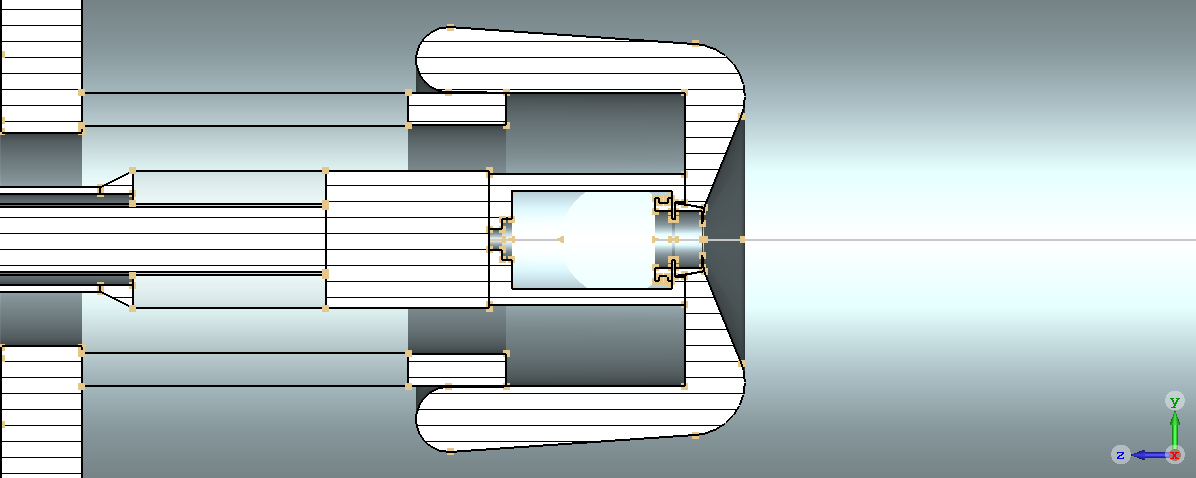
\includegraphics[width=\textwidth]{figures/200kV/v1_cutx}
  \caption{$y$-$z$ view of the CST model for $x=0$.}
  \label{fig:cst_geometry_yz}
\end{figure}
\end{center}

\begin{center}
\begin{figure}[H]
  \begin{tikzpicture}
\begin{axis}[
   scale only axis = true,
   width = 0.9\textwidth,
  axis equal,
  try min ticks=4,
  max space between ticks=1000pt,
  enlargelimits=true,
  colormap/Greens,
  point meta min = 0,
  point meta max = 2,
  x unit=m,
  y unit=m]

  \addplot[surf, shader=interp] table[point meta=\thisrow{c}]{figures/200kV/geometry/geometry_1.dat};

  \addplot[surf, shader=interp] table[point meta=\thisrow{c}]{figures/200kV/geometry/geometry_2.dat};

  \addplot[surf, shader=interp] table[point meta=\thisrow{c}]{figures/200kV/geometry/geometry_3.dat};

  \addplot[surf, shader=interp] table[point meta=\thisrow{c}]{figures/200kV/geometry/geometry_4.dat};

  \addplot[surf, shader=interp] table[point meta=\thisrow{c}]{figures/200kV/geometry/geometry_5.dat};

  \addplot[surf, shader=interp] table[point meta=\thisrow{c}]{figures/200kV/geometry/geometry_6.dat};

  \addplot[surf, shader=interp] table[point meta=\thisrow{c}]{figures/200kV/geometry/geometry_7.dat};

  \addplot[surf, shader=interp] table[point meta=\thisrow{c}]{figures/200kV/geometry/geometry_8.dat};

  \addplot[surf, shader=interp] table[point meta=\thisrow{c}]{figures/200kV/geometry/geometry_9.dat};

  \addplot[surf, shader=interp] table[point meta=\thisrow{c}]{figures/200kV/geometry/geometry_10.dat};

  \addplot[surf, shader=interp] table[point meta=\thisrow{c}]{figures/200kV/geometry/geometry_11.dat};

  \addplot[surf, shader=interp] table[point meta=\thisrow{c}]{figures/200kV/geometry/geometry_12.dat};

  \addplot[surf, shader=interp] table[point meta=\thisrow{c}]{figures/200kV/geometry/geometry_13.dat};

  \addplot[surf, shader=interp, colormap/Reds, point meta min = 0, point meta max = 1] table[point meta=\thisrow{c}]{figures/200kV/geometry/geometry_13.dat};

  \addplot[surf, shader=interp] table[point meta=\thisrow{c}]{figures/200kV/geometry/geometry_14.dat};

  \addplot[surf, shader=interp] table[point meta=\thisrow{c}]{figures/200kV/geometry/geometry_15.dat};

  \addplot[surf, shader=interp, colormap/Reds, point meta min = 0, point meta max = 1] table[point meta=\thisrow{c}]{figures/200kV/geometry/geometry_16.dat};

  \addplot[surf, shader=interp, colormap/Reds, point meta min = 0, point meta max = 1] table[point meta=\thisrow{c}]{figures/200kV/geometry/geometry_17.dat};

  \addplot[surf, shader=interp] table[point meta=\thisrow{c}]{figures/200kV/geometry/geometry_18.dat};

  \addplot[surf, shader=interp] table[point meta=\thisrow{c}]{figures/200kV/geometry/geometry_19.dat};

  \addplot[surf, shader=interp] table[point meta=\thisrow{c}]{figures/200kV/geometry/geometry_20.dat};

  \addplot[surf, shader=interp] table[point meta=\thisrow{c}]{figures/200kV/geometry/geometry_21.dat};

  \addplot[surf, shader=interp] table[point meta=\thisrow{c}]{figures/200kV/geometry/geometry_22.dat};

  % add patch indices
  \addplot[only marks, point meta=explicit symbolic, color=black, nodes near coords] coordinates{
  (0.28,-0.01) [(1)]
  (0.28,-0.005) [(2)]
  (0.28,0.005) [(3)]
  (0.28,0.015) [(4)]
  (0.28,0.045) [(5)]
  (0.24,0.075) [(6)]
  (0.15,0.075) [(7)]
  (0.085,0.075) [(8)]
  (0.1,0.05) [(9)]
  (0.05,0.065) [(10)]
  (0.1,0.04) [(11)]
  (0.05,0.045) [(12)]
  (0.05,0.03) [(13)]
  (0.03,0.0175) [(14)]
  (0.0075,0.0075) [(15)]
  (0.04,0.007) [(16)]
  (0.0075,0.0025) [(17)]
  (0.075,0.017) [(18)]
  (0.115,0.017) [(19)]
  (0.135,0.015) [(20)]
  (0.155,0.025) [(21)]
  (0.035,-0.005) [(22)]
  };

  % add patch boundaries
  \addplot[color=brewerblue] table{figures/200kV/boundary/boundaries11.dat};
  \addplot[color=brewerred] table{figures/200kV/boundary/boundaries12.dat};
  \addplot[color=black] table{figures/200kV/boundary/boundaries13.dat};
  \addplot[color=brewergrey] table{figures/200kV/boundary/boundaries14.dat};

  \addplot[color=brewerblue] table{figures/200kV/boundary/boundaries21.dat};
  \addplot[color=brewerred] table{figures/200kV/boundary/boundaries22.dat};
  \addplot[color=brewergrey] table{figures/200kV/boundary/boundaries23.dat};
  \addplot[color=brewergrey] table{figures/200kV/boundary/boundaries24.dat};

  \addplot[color=brewerblue] table{figures/200kV/boundary/boundaries31.dat};
  \addplot[color=brewerred] table{figures/200kV/boundary/boundaries32.dat};
  \addplot[color=brewergrey] table{figures/200kV/boundary/boundaries33.dat};
  \addplot[color=brewergrey] table{figures/200kV/boundary/boundaries34.dat};

  \addplot[color=brewerblue] table{figures/200kV/boundary/boundaries41.dat};
  \addplot[color=brewerred] table{figures/200kV/boundary/boundaries42.dat};
  \addplot[color=brewergrey] table{figures/200kV/boundary/boundaries43.dat};
  \addplot[color=brewergrey] table{figures/200kV/boundary/boundaries44.dat};

  \addplot[color=brewerblue] table{figures/200kV/boundary/boundaries51.dat};
  \addplot[color=brewerred] table{figures/200kV/boundary/boundaries52.dat};
  \addplot[color=brewergrey] table{figures/200kV/boundary/boundaries53.dat};
  \addplot[color=brewergrey] table{figures/200kV/boundary/boundaries54.dat};

  \addplot[color=brewerblue] table{figures/200kV/boundary/boundaries61.dat};
  \addplot[color=brewerred] table{figures/200kV/boundary/boundaries62.dat};
  \addplot[color=brewergrey] table{figures/200kV/boundary/boundaries63.dat};
  \addplot[color=brewergrey] table{figures/200kV/boundary/boundaries64.dat};

  \addplot[color=brewerblue] table{figures/200kV/boundary/boundaries71.dat};
  \addplot[color=brewerred] table{figures/200kV/boundary/boundaries72.dat};
  \addplot[color=brewergrey] table{figures/200kV/boundary/boundaries73.dat};
  \addplot[color=brewergrey] table{figures/200kV/boundary/boundaries74.dat};

  \addplot[color=brewergrey] table{figures/200kV/boundary/boundaries81.dat};
  \addplot[color=brewerred] table{figures/200kV/boundary/boundaries82.dat};
  \addplot[color=brewergrey] table{figures/200kV/boundary/boundaries83.dat};
  \addplot[color=brewergrey] table{figures/200kV/boundary/boundaries84.dat};

  \addplot[color=brewergrey] table{figures/200kV/boundary/boundaries91.dat};
  \addplot[color=brewerblue] table{figures/200kV/boundary/boundaries92.dat};
  \addplot[color=brewergrey] table{figures/200kV/boundary/boundaries93.dat};
  \addplot[color=brewergrey] table{figures/200kV/boundary/boundaries94.dat};

  \addplot[color=brewerred] table{figures/200kV/boundary/boundaries101.dat};
  \addplot[color=brewergrey] table{figures/200kV/boundary/boundaries102.dat};
  \addplot[color=brewergrey] table{figures/200kV/boundary/boundaries103.dat};
  \addplot[color=brewergrey] table{figures/200kV/boundary/boundaries104.dat};

  \addplot[color=brewergrey] table{figures/200kV/boundary/boundaries111.dat};
  \addplot[color=brewerblue] table{figures/200kV/boundary/boundaries112.dat};
  \addplot[color=brewerblue] table{figures/200kV/boundary/boundaries113.dat};
  \addplot[color=brewergrey] table{figures/200kV/boundary/boundaries114.dat};

  \addplot[color=brewerred] table{figures/200kV/boundary/boundaries121.dat};
  \addplot[color=brewergrey] table{figures/200kV/boundary/boundaries122.dat};
  \addplot[color=brewergrey] table{figures/200kV/boundary/boundaries123.dat};
  \addplot[color=brewergrey] table{figures/200kV/boundary/boundaries124.dat};

  \addplot[color=brewerred] table{figures/200kV/boundary/boundaries131.dat};
  \addplot[color=brewerblue] table{figures/200kV/boundary/boundaries132.dat};
  \addplot[color=brewergrey] table{figures/200kV/boundary/boundaries133.dat};
  \addplot[color=brewergrey] table{figures/200kV/boundary/boundaries134.dat};

  \addplot[color=brewerred] table{figures/200kV/boundary/boundaries141.dat};
  \addplot[color=brewergrey] table{figures/200kV/boundary/boundaries142.dat};
  \addplot[color=brewergrey] table{figures/200kV/boundary/boundaries143.dat};
  \addplot[color=brewergrey] table{figures/200kV/boundary/boundaries144.dat};

  \addplot[color=brewerred] table{figures/200kV/boundary/boundaries151.dat};
  \addplot[color=brewergrey] table{figures/200kV/boundary/boundaries152.dat};
  \addplot[color=brewergrey] table{figures/200kV/boundary/boundaries153.dat};
  \addplot[color=brewergrey] table{figures/200kV/boundary/boundaries154.dat};

  \addplot[color=brewergrey] table{figures/200kV/boundary/boundaries161.dat};
  \addplot[color=brewerblue] table{figures/200kV/boundary/boundaries162.dat};
  \addplot[color=brewergrey] table{figures/200kV/boundary/boundaries163.dat};
  \addplot[color=brewergrey] table{figures/200kV/boundary/boundaries164.dat};

  \addplot[color=brewerred] table{figures/200kV/boundary/boundaries171.dat};
  \addplot[color=brewergrey] table{figures/200kV/boundary/boundaries172.dat};
  \addplot[color=brewergrey] table{figures/200kV/boundary/boundaries173.dat};
  \addplot[color=brewergrey] table{figures/200kV/boundary/boundaries174.dat};

  \addplot[color=brewergrey] table{figures/200kV/boundary/boundaries181.dat};
  \addplot[color=brewergrey] table{figures/200kV/boundary/boundaries182.dat};
  \addplot[color=brewergrey] table{figures/200kV/boundary/boundaries183.dat};
  \addplot[color=brewerblue] table{figures/200kV/boundary/boundaries184.dat};

  \addplot[color=brewergrey] table{figures/200kV/boundary/boundaries191.dat};
  \addplot[color=brewergrey] table{figures/200kV/boundary/boundaries192.dat};
  \addplot[color=brewerblue] table{figures/200kV/boundary/boundaries193.dat};
  \addplot[color=brewerblue] table{figures/200kV/boundary/boundaries194.dat};

  \addplot[color=brewerblue] table{figures/200kV/boundary/boundaries201.dat};
  \addplot[color=brewergrey] table{figures/200kV/boundary/boundaries202.dat};
  \addplot[color=brewerblue] table{figures/200kV/boundary/boundaries203.dat};
  \addplot[color=brewergrey] table{figures/200kV/boundary/boundaries204.dat};

  \addplot[color=brewerblue] table{figures/200kV/boundary/boundaries211.dat};
  \addplot[color=brewerblue] table{figures/200kV/boundary/boundaries212.dat};
  \addplot[color=brewergrey] table{figures/200kV/boundary/boundaries213.dat};
  \addplot[color=brewerblue] table{figures/200kV/boundary/boundaries214.dat};

  \addplot[color=brewerred] table{figures/200kV/boundary/boundaries221.dat};
  \addplot[color=brewerblue] table{figures/200kV/boundary/boundaries222.dat};
  \addplot[color=black] table{figures/200kV/boundary/boundaries223.dat};
  \addplot[color=brewergrey] table{figures/200kV/boundary/boundaries224.dat};
\end{axis}
\end{tikzpicture}

  \caption{200 kV Photocathode geometry and boundary conditions.}
  \label{fig:200kV_geometry}
\end{figure}
\end{center}

\begin{center}
\begin{figure}[H]
  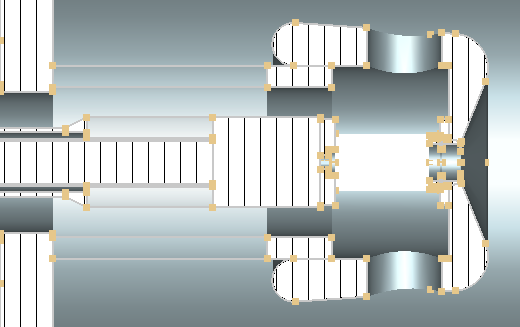
\includegraphics[width=\textwidth]{figures/200kV/v1_cuty}
  \caption{$x$-$z$ view of the CST model for $y=0$.}
  \label{fig:cst_geometry_xz}
\end{figure}
\end{center}

\subsection{Electrostatic Potential and Electric Field}
The solution for the electrostatic potential is shown in fig.~\ref{fig:200kV_potential}. Fig.~\ref{fig:200kV_electric_field} depicts the absolute value of the electric field.
Both of the solutions were computed with $p=4$ as the degree of the basis functions and $n_\mathrm{sub}=128$ as the number of elements that each knot vector is uniformly split into.
It is evident that there exist parts of the domain where the magnitude exceeds the limit of $10 \frac{\mathrm{MV}}{\mathrm{m}}$. There are also very high gradients visible at the triple points however these also coincide with sharp corners so numerical issues might play a role. (Again perform a convergence study and investigate the absolute error per patch?)

\begin{center}
\begin{figure}[H]
  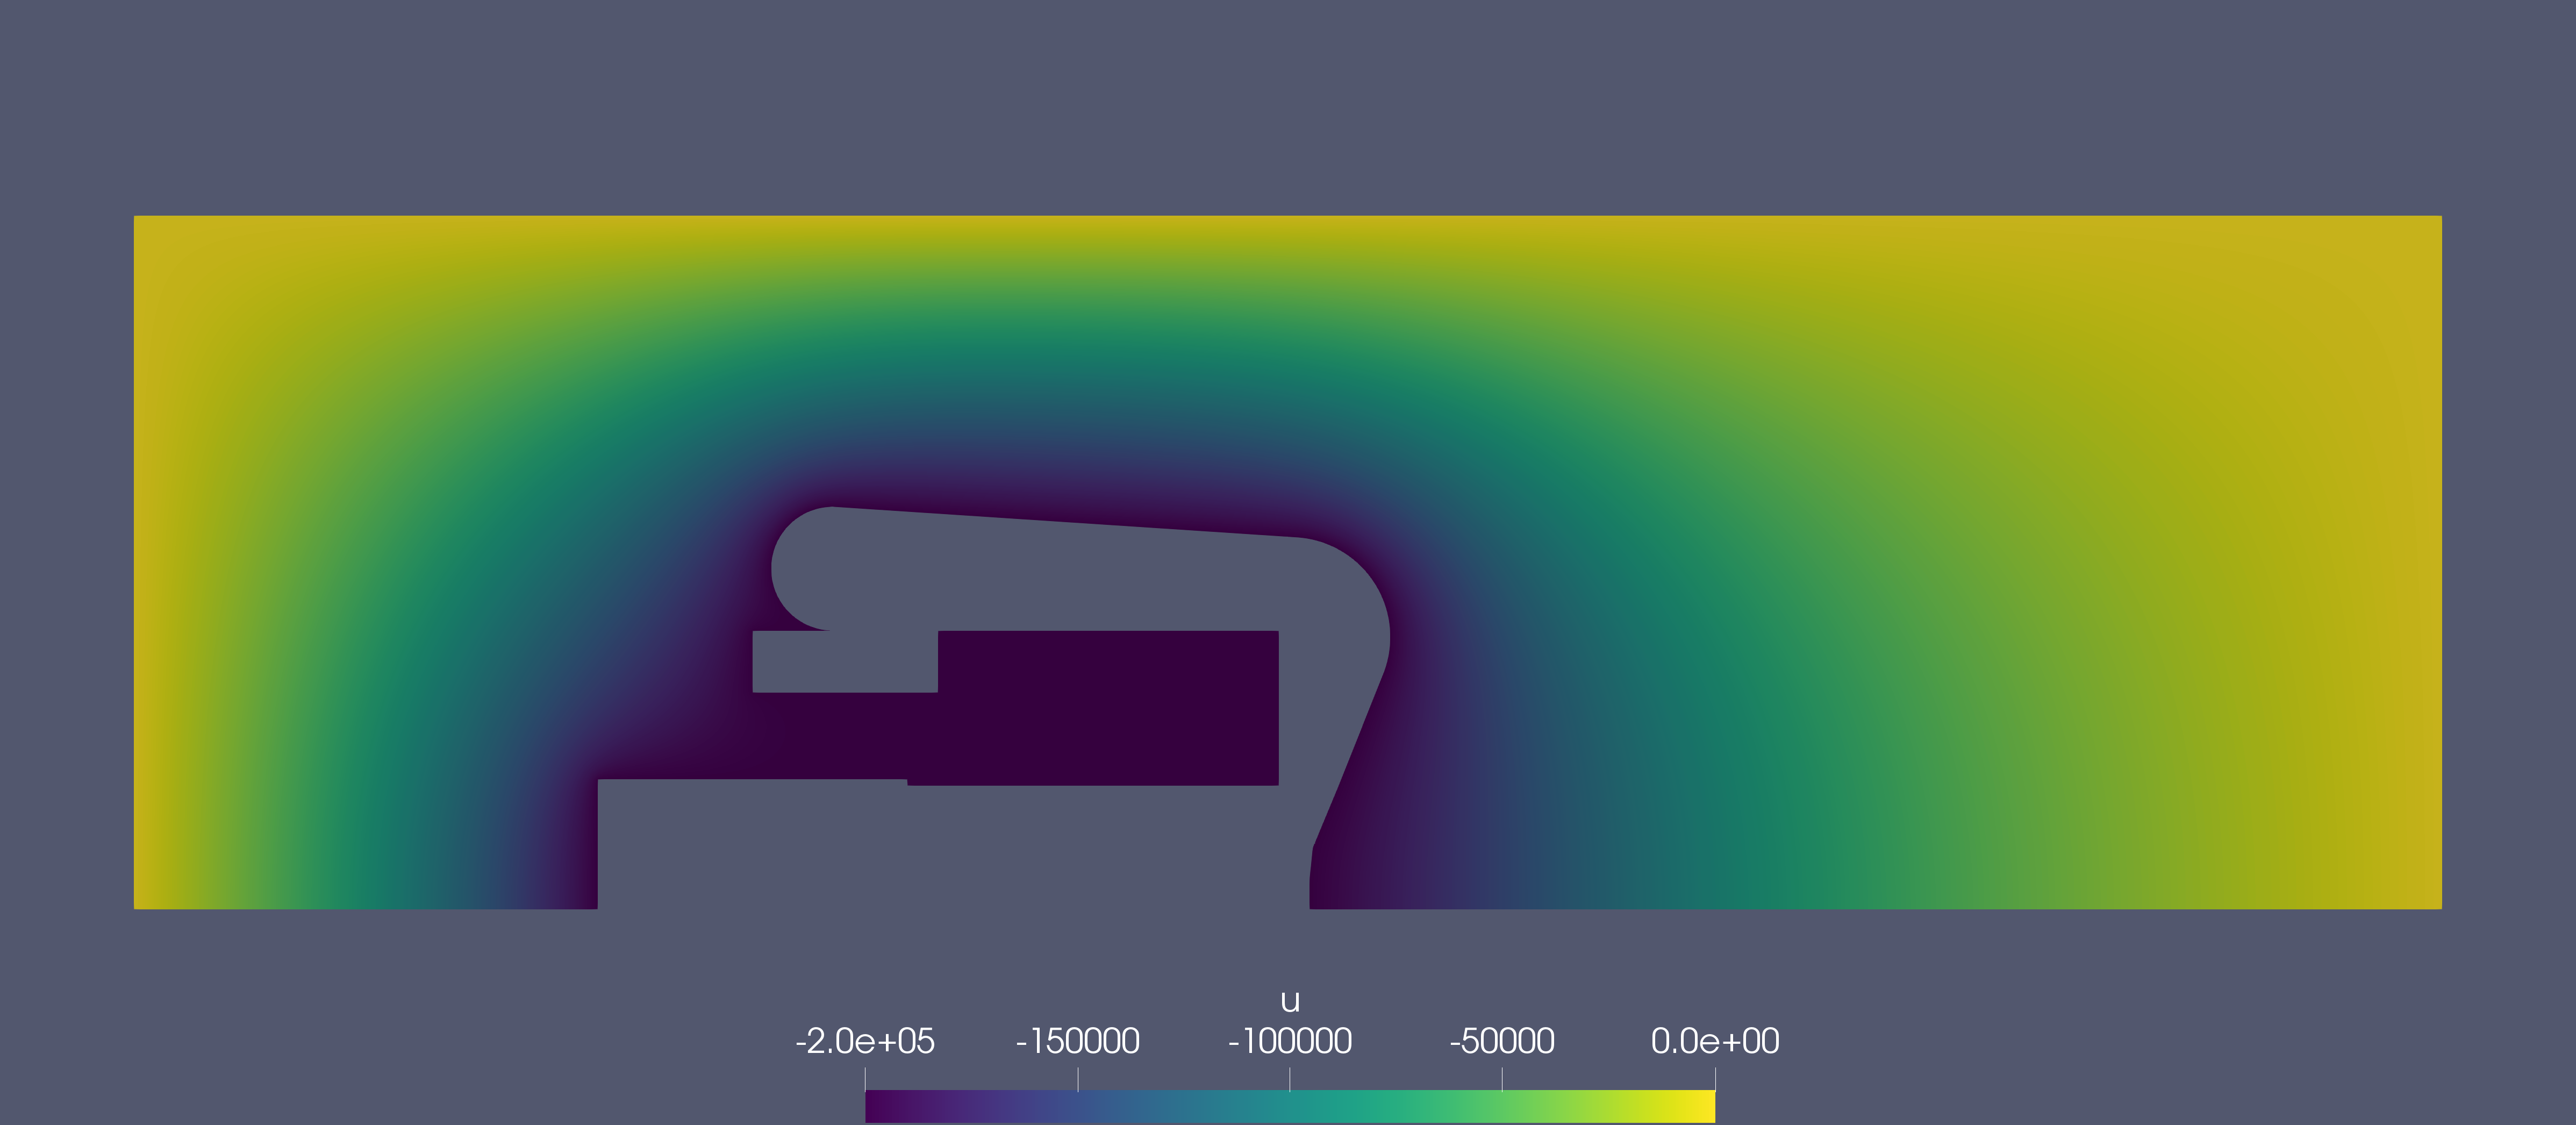
\includegraphics[width=\textwidth]{figures/200kV/potential}
  \caption{Electrostatic potential.}
  \label{fig:200kV_potential}
\end{figure}
\end{center}

\begin{center}
\begin{figure}[H]
  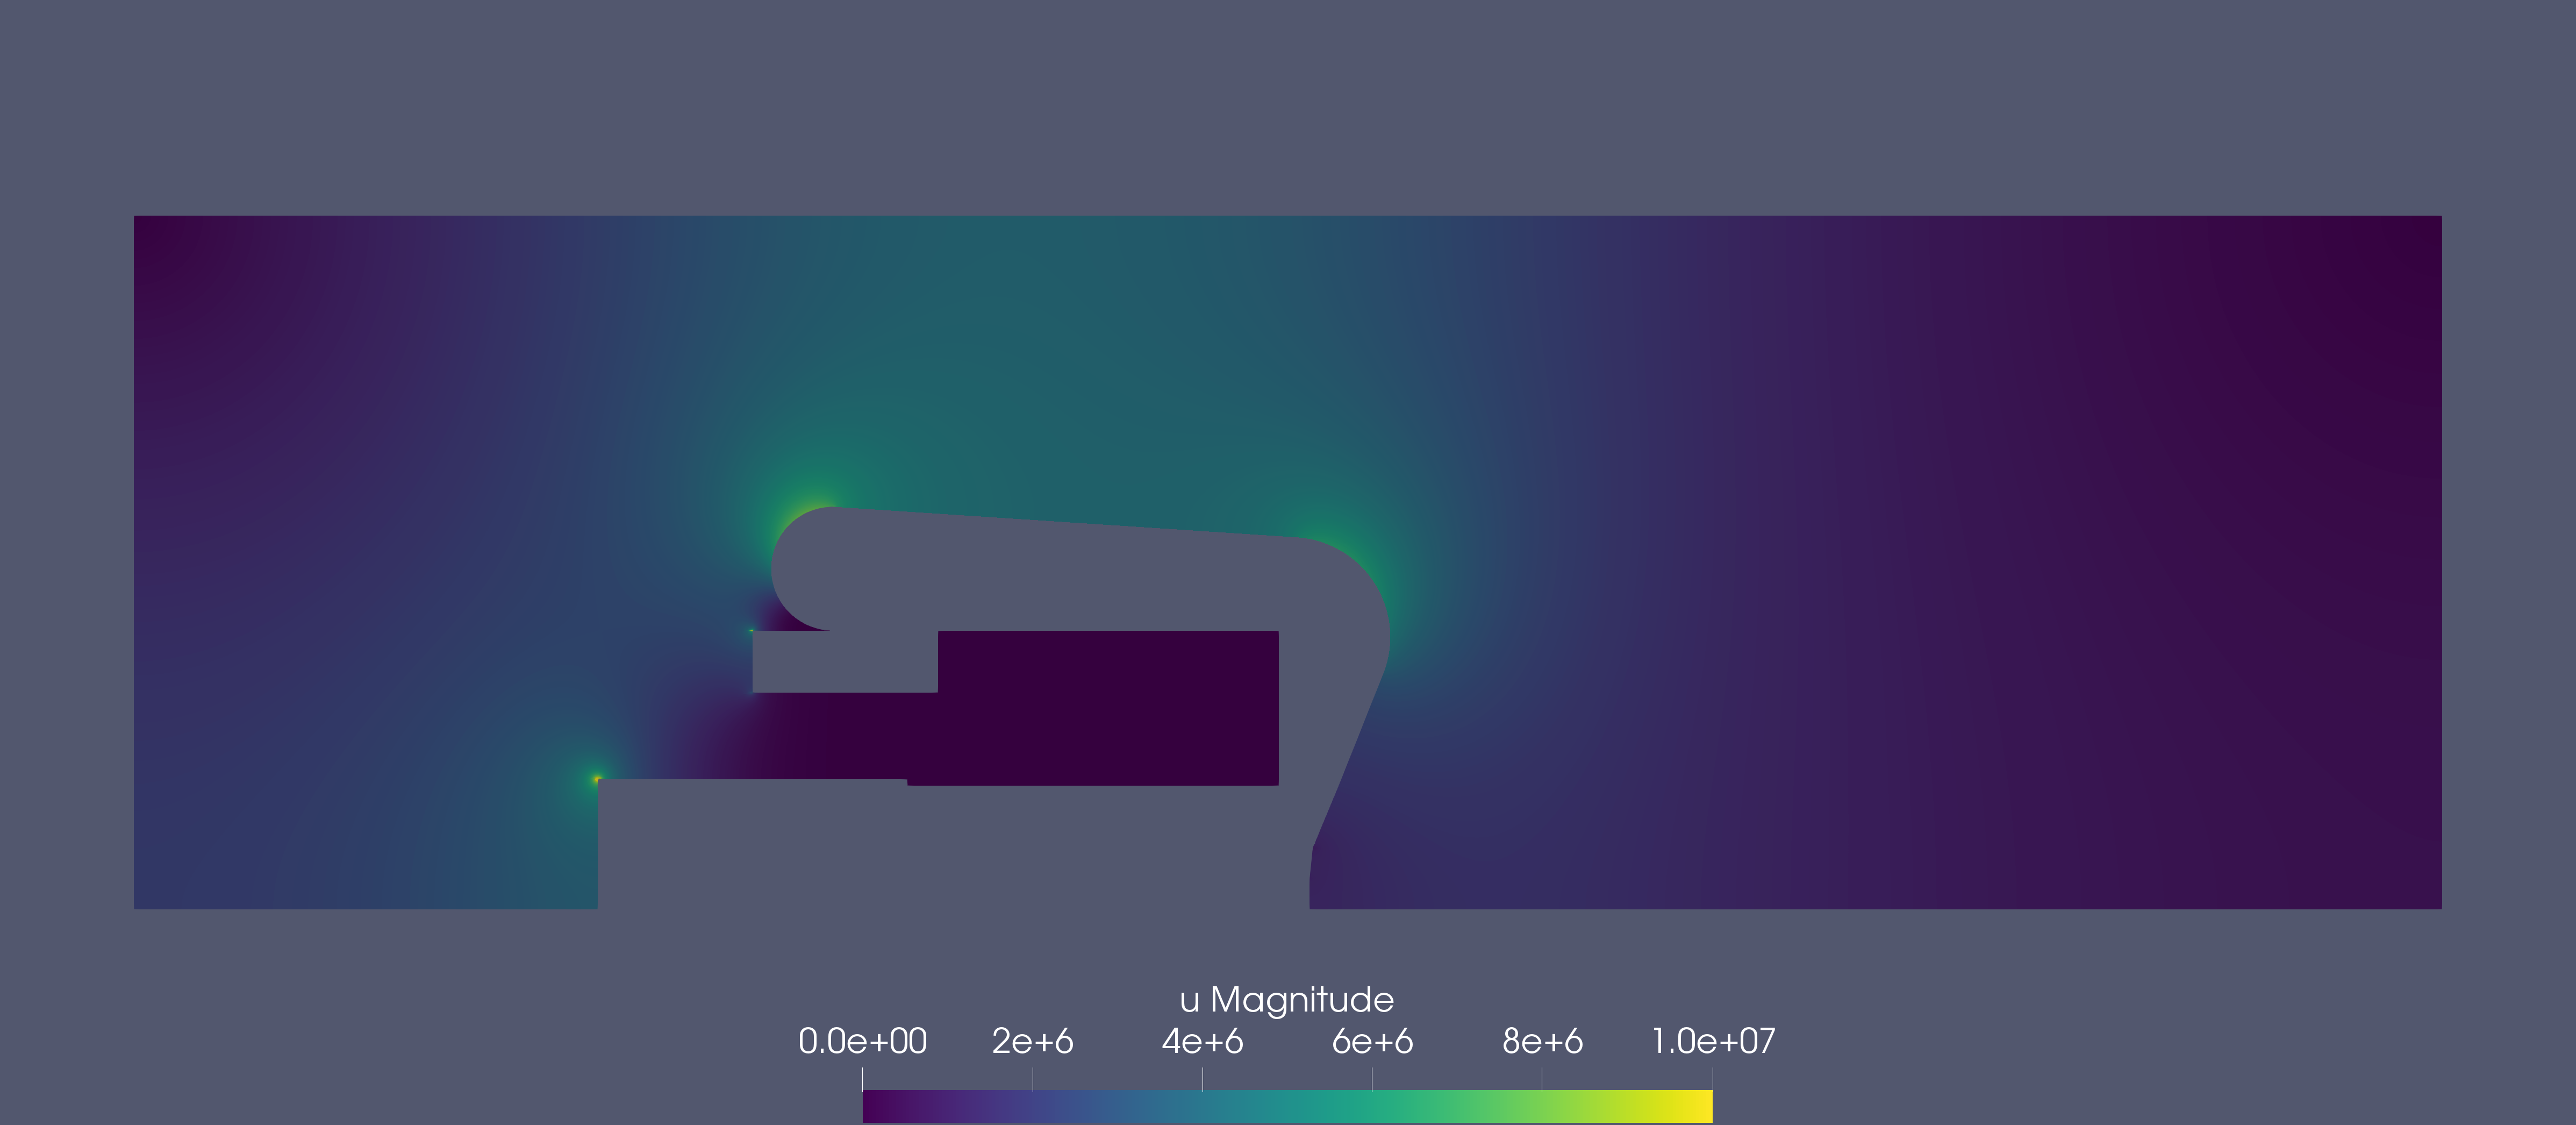
\includegraphics[width=\textwidth]{figures/200kV/gradient}
  \caption{Absolute value of the electric field.}
  \label{fig:200kV_electric_field}
\end{figure}
\end{center}

\subsection{Optimization}
The aim of the optimization will be to minimize the maximal field amplitudes. For practicality we will only look at the critical points of the geometry, i.~e.~the curvatures of the outer electrode and the triple points and average the field strengths over a given number of sample points. The lower part of the geometry will remain fixed so only the electrode boundaries of patches 5, 6, 7, 8, 9 and 11 from fig.~\ref{fig:200kV_geometry} and their respective control points will be the DoFs. Another thing that might be considered is varying the length of the entire electrode. Aside from the fixed part of the geometry we also need to consider the volume constraint as stated previously.

\subsubsection{Volume Constraint}
One of the constraints for the later optimization will be the weight of the electrode and thus its volume.
We first compute the volume of the patches by taking into account the rotational symmetry and discretizing $V_{\mathrm{ptc}} = \int_V r\ \drm r\ \drm \varphi\ \drm z$ via numerical quadrature. We can then obtain the volume of the electrode by subtracting $V_{\mathrm{ptc}}$ from the cylinder formed by the vacuumchamber.
For the discretization we have
\begin{align}
   V_{\mathrm{ptc}} = \int_V r\ \drm r\ \drm \varphi\ \drm z \approx \sum_{i=1}^n \wbf_{z_i} (\Wbf_x(z_i) \Wbf_y(z_i))
\end{align}
where we discretized $z$ with $n$ quadrature points.
We still need to consider the holes inside the electrode and the correct lift geometry. The holes are computed by considering a cylinder with its height as a function of $z$. The curvature in $x$ and $y$ is disregarded, since it is the same for both coordinates. We can therefore determine the value by discretizing $V_{h} = \int_V \drm x\ \drm y\ \drm z$.
Lastly the puck lift is made up mostly of vacuum. Its shape can be decomposed into two cylinders and two cylinder parts, which can be computed by the same approach used for the holes.

$\rho = 7.99 \frac{\mathrm{g}}{\mathrm{mm}^3}$

\subsection{Astra}
In the future we may also optimize the electrode boundary next to the puck, i.~e.~patches 2, 3 and 4 to obtain optimal particle trajectories. The cost function will be computed using Astra. (Perform all the tests for Astra also for the final Photocathode geometry?)
The desired total bunch charge is $10$ pC with a beam current of $(20-100)\ \mu\mathrm{A}$, whereas a typical value would be $100$ fC. The bunch length is around $5$ ps with a normalized transversal emittance of $e_{x,y} \leq 1\ \mathrm{mm\ mrad}$. The desired energy resolution is $\frac{\Delta E}{E} \leq 10^{-4}$.
The tracking will be performed using individual bunches from a pulsed laser. The emission model may be derived from \cite{wagner}.
